\documentclass[letterpaper,twocolumn,10pt]{article}
\usepackage{usenix,epsfig,endnotes}
\usepackage{xcolor}
\usepackage{booktabs}
\usepackage{tabularx}
\usepackage[labelfont=bf,textfont=bf]{caption}
\captionsetup{hypcap=false,skip=4pt}
\usepackage{tikz}
\usetikzlibrary{arrows.meta,positioning,fit,backgrounds}
\usepackage{pgfplots}
\pgfplotsset{compat=1.18}
\usepackage{algorithm}
\usepackage{algpseudocode}

\begin{document}

%don't want date printed
\date{}

%make title bold and 14 pt font (Latex default is non-bold, 16 pt)
\title{\Large \bf LLM-Guided Rule Discovery for Web Attack Detection}

\author{
{\rm Rahul Tripathi}\\
UCLA
\and
{\rm Armaan Oberai}\\
UCLA
\and
{\rm Justine Ellery}\\
UCLA
}

\pagenumbering{gobble}
\begin{titlepage}
\centering
\vspace*{1.25in}
{\Large \bf LLM-Guided Rule Discovery for Web Attack Detection\par}
\vspace{0.35in}
{\large ECE239AS Network Security Final Report\par}
\vspace{0.25in}
{\large Team: LLM-Guided Rules\par}
\vspace{0.5in}
\begin{tabular}{ll}
Rahul Tripathi & \texttt{rahultripathi1@g.ucla.edu} \\
Armaan Oberai & \texttt{aoberai123@g.ucla.edu} \\
Justine Ellery & \texttt{justineellery@g.ucla.edu} \\
\end{tabular}
\vfill
{\large UCLA\par}
\end{titlepage}
\clearpage
\pagenumbering{arabic}

\maketitle

% Use the following at camera-ready time to suppress page numbers.
% Comment it out when you first submit the paper for review.
\thispagestyle{empty}


\subsection*{Abstract}

Web-application attacks often leave textual and structural evidence in HTTP requests, but turning that evidence into deployable rules remains difficult. Machine-learning models can classify benchmark traffic accurately, yet they usually produce model artifacts rather than compact detection logic that operators can inspect and revise. This paper studies whether an LLM can help discover simple web-attack rules without becoming the runtime detector. We build a Python harness that uses an LLM-guided process to propose regexes and endpoint heuristics, then evaluates each candidate with deterministic precision and recall checks. On a stratified 80/20 split of CSIC 2010, the frozen rule set reaches 99.21\% test accuracy and 0.9903 F1, exceeding the reproduced random-forest machine-learning baseline on the same split. The final output is a compact rule set rather than a trained model, making it easier to translate into rule-based firewall or WAF-style enforcement pipelines than a traditional machine-learning classifier.

\section{Introduction}

Web attacks often reveal themselves in the text of an HTTP request. A SQL injection attempt may introduce quotes, comments, or database keywords; a cross-site scripting attempt may introduce markup or encoded script fragments; a malformed request may mutate a parameter name that is otherwise stable for an endpoint. These signals are not proof that every attack can be captured by a simple signature. However, they show why web-attack detection has long relied on rules: many attacks expose service-visible clues that a deterministic detector can inspect directly.

Rules matter because web defenses often sit directly on the request path. A web application firewall must inspect many requests before they reach the application, and widely deployed systems such as ModSecurity are built around rule engines and generic rule sets such as the OWASP Core Rule Set~\cite{OWASPModSecurity,OWASPCoreRuleSet}. This design reflects an operational constraint: detection logic must be fast, predictable, and cheap enough to run continuously. IDS surveys make the same point for network settings, where detectors must handle high-volume streams under real-time, high-dimensionality, and computational-efficiency constraints~\cite{Adnan2021IoTIDSReview}. Dense models may be useful offline or as a secondary signal, but they are harder to justify as the only mechanism when every request must be inspected at line rate.

Machine-learning models show that web attacks are learnable, but they do not directly produce deployable detection logic. On CSIC 2010, a common web-application intrusion-detection benchmark, random forests over character TF-IDF features can classify attacks with high accuracy. This is useful evidence that request text contains enough structure to separate normal and anomalous traffic. Yet the output is a trained model rather than a compact explanation of which request patterns matter. For operators who need to audit, revise, and deploy detection logic, model accuracy alone does not solve the rule-writing problem.

Manual rule writing does not scale to the variation present even in a small benchmark. A rule that flags encoded script tags may catch many XSS examples, but it will miss attacks expressed as endpoint-specific parameter mutations, malformed numeric fields, or unusual but valid encodings. Conversely, a broad rule can quickly produce false positives on benign strings such as product names, addresses, or passwords. The problem is therefore not simply to write more regexes. It is to discover candidate rules, measure their marginal value, and reject rules that overfit or duplicate existing behavior.

This paper explores whether an LLM can help discover HTTP attack rules without becoming the detector. We use the LLM as an offline proposal mechanism that suggests regexes and endpoint-specific heuristics. A deterministic harness executes each candidate rule, measures its effect on false positives and false negatives, and keeps only rules that improve measured precision and recall. The final detector contains no LLM calls and does not depend on a production IDS rule language. It is a compact Python rule set whose behavior can be inspected request by request.

We evaluate this idea on the CSIC 2010 web-application attack dataset. CSIC 2010 contains 36{,}000 normal requests and 25{,}065 anomalous requests from a synthetic e-commerce application, including SQL injection, cross-site scripting, CRLF injection, buffer overflow, information-gathering, and malformed-request attacks. We first reproduce a machine-learning baseline based on character TF-IDF and tree models, then build a rule-discovery harness over raw and decoded request fields. On the same stratified 80/20 split used by the baseline, the frozen rules reach 99.21\% test accuracy and evaluate all 61{,}065 requests in about 2.8 seconds. This suggests that compact rules can recover much of the performance of a strong statistical baseline while remaining auditable.

Our contribution is a controlled methodology for LLM-guided rule discovery. Rather than treating the LLM as a classifier, we separate proposal, execution, evaluation, and acceptance. Rather than generating Suricata or ModSecurity signatures, we study a deliberately small rule language of Python regexes and endpoint heuristics. We report performance on the same stratified 80/20 train/test split used by the reproduced machine-learning baseline. This setup asks a narrow question: when web-attack patterns are visible in request text, can an LLM-guided loop recover accurate, fast, and auditable detection logic?

\section{Background and Related Work}

Web-attack detection is often evaluated on small, structured benchmarks whose attacks are visible in HTTP request text. Early intrusion-detection datasets, including the DARPA collections, were important but poorly matched to web-application attacks because they contained unrealistic traffic and limited HTTP attack coverage~\cite{McHugh2000Critique}. CSIC 2010 was created to address this gap with traffic from a synthetic e-commerce application~\cite{CSIC2010}. The dataset contains more than 36{,}000 normal HTTP requests and more than 25{,}000 anomalous requests, including SQL injection, cross-site scripting, buffer overflow, CRLF injection, information-gathering, and malformed-request attacks. As a result, CSIC 2010 has become a common benchmark for web-application intrusion detection.

Machine-learning models can classify CSIC 2010 accurately, but they do not produce simple detection logic. Prior work has applied statistical anomaly detectors, tree ensembles, and deep neural models to HTTP or network intrusion detection~\cite{Lampesberger2012Online,Adewole2025IDS,Odumuyiwa2021HTTPInjection,Wang2024CCBA}. These systems can learn lexical and structural regularities in request data, and strong baselines on CSIC 2010 use character TF-IDF features with random forests or gradient boosting~\cite{MustafaKaggleNotebook}. However, the resulting detector is usually a model artifact rather than a compact rule set that an analyst can inspect, edit, or deploy as a simple signature engine. Extracted tree rules improve transparency only partially because the induced rules are often numerous and unstable.

LLM-based intrusion detection has mostly used language models as flexible classifiers or payload interpreters. Recent systems integrate LLMs into NetFlow, packet-payload, or hybrid signature pipelines to reduce false positives and catch patterns missed by fixed rules~\cite{Davey2025LLMIDS,AlHammouri2025Hybrid}. This use of LLMs is attractive because attack evidence is often textual and irregular. However, the final decision often remains a model judgment rather than a durable detection artifact. For web-attack detection, this leaves the same gap as earlier machine-learning systems: high-level accuracy does not necessarily yield auditable rules.

LLM-assisted rule generation is closer to our goal because it uses models to produce interpretable artifacts. Recent systems generate Suricata, Snort, ModSecurity, KQL, or other detection rules from traffic captures, threat intelligence, or natural-language descriptions~\cite{Roesch1999Snort,Suricata,ModSecurity,KQL,Moreno2025LLMRuleGen,Li2025GRIDAI,Fu2026VibeWAF,Meng2026UniRule,Wang2025RulePilot,Konstantaras2026EDR}. These systems commonly pair generation with automated evaluation or repair so that invalid rules can be rejected. They also show two recurring challenges: generated rules are tied to complex target languages, and online rule-generation systems can accumulate redundant or unbounded rule sets. This makes it harder to isolate a simpler question: can an LLM help discover compact HTTP rules over a fixed benchmark?

Our work studies a smaller and more controlled form of rule discovery. Unlike machine-learning and deep-learning detectors, our output is not a model that directly classifies requests. Unlike LLM-as-detector systems, the LLM is not part of the runtime detection path. Unlike LLM rule-generation systems for Suricata, ModSecurity, or KQL, our target language is deliberately minimal: Python regexes and endpoint heuristics. This lets us ask whether an LLM-guided search loop can discover compact, auditable HTTP attack rules without inheriting the complexity of a full IDS rule language.

Our harness treats the LLM as an offline proposal mechanism rather than as the detector. The LLM proposes candidate rules, but a deterministic evaluator executes them and accepts them only when they improve detection under explicit precision and recall constraints. The same held-out test split used by the reproduced baseline is used for reporting the frozen detector. This separates rule discovery from rule execution and makes every retained rule inspectable. The core question is therefore not whether LLMs can classify attacks, but whether they can help discover simple rules that recover much of the performance of statistical models on a web-attack benchmark.

\section{Methodology}

Our methodology separates rule discovery from rule execution. The LLM is used only during an offline search loop, where it proposes candidate regexes and endpoint heuristics from examples and error summaries. A deterministic harness then executes those candidates, measures their effect on classification behavior, and decides whether to retain them. The final detector is therefore not an LLM classifier. It is a fixed rule set that can be run, inspected, and revised without calling a model.

\begin{figure}[t]
\centering
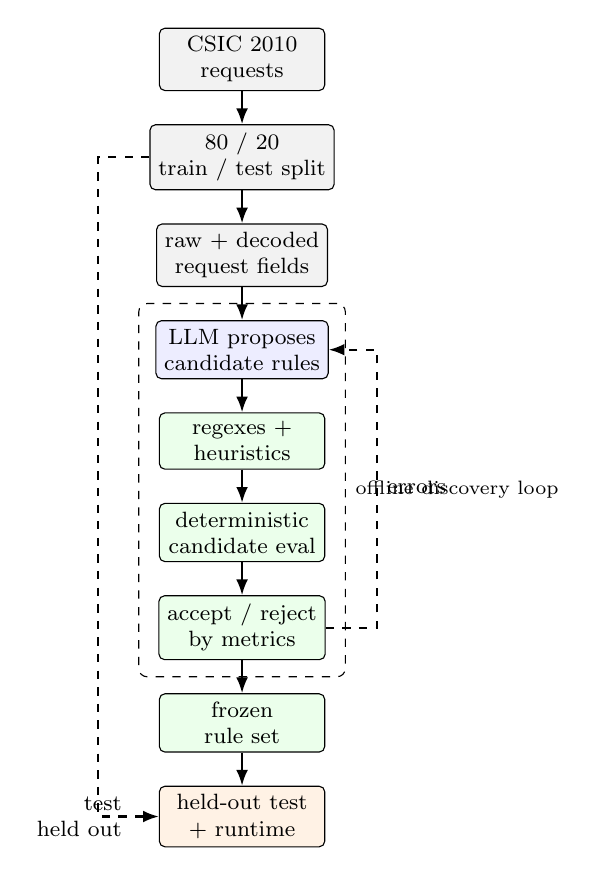
\begin{tikzpicture}[
    font=\footnotesize,
    node distance=0.42cm and 0.55cm,
    box/.style={
        draw,
        rounded corners=2pt,
        align=center,
        minimum width=2.1cm,
        minimum height=0.56cm,
        inner sep=3pt
    },
    data/.style={box, fill=gray!10},
    model/.style={box, fill=blue!7},
    eval/.style={box, fill=green!8},
    test/.style={box, fill=orange!10},
    arrow/.style={-{Latex[length=2mm]}, thick},
    dashedarrow/.style={-{Latex[length=2mm]}, thick, dashed}
]
\node[data] (dataset) {CSIC 2010\\requests};
\node[data, below=of dataset] (split) {80 / 20\\train / test split};
\node[data, below=of split] (repr) {raw + decoded\\request fields};

\node[model, below=of repr] (llm) {LLM proposes\\candidate rules};
\node[eval, below=of llm] (candidate) {regexes +\\heuristics};
\node[eval, below=of candidate] (eval) {deterministic\\candidate eval};
\node[eval, below=of eval] (accept) {accept / reject\\by metrics};
\node[eval, below=of accept] (rules) {frozen\\rule set};
\node[test, below=of rules] (final) {held-out test\\+ runtime};

\draw[arrow] (dataset) -- (split);
\draw[arrow] (split) -- (repr);
\draw[arrow] (repr) -- (llm);
\draw[arrow] (llm) -- (candidate);
\draw[arrow] (candidate) -- (eval);
\draw[arrow] (eval) -- (accept);
\draw[arrow] (accept) -- (rules);
\draw[arrow] (rules) -- (final);
\draw[dashedarrow] (accept.east) -- ++(0.65,0) |- node[pos=0.25, right, align=left] {errors} (llm.east);
\draw[dashedarrow] (split.west) -- ++(-0.65,0) |- node[pos=0.78, left, align=right] {test\\held out} (final.west);

\begin{scope}[on background layer]
\node[draw, dashed, rounded corners=3pt, fit=(llm)(candidate)(eval)(accept), inner sep=6pt, label={[font=\scriptsize]right:offline discovery loop}] {};
\end{scope}
\end{tikzpicture}
\caption{Proposal Is Separate From Detection --- The agent-guided loop uses the LLM only to propose candidate regexes and heuristics from examples and error summaries. A deterministic evaluator accepts only rules that improve measured metrics, and the frozen rule set is reported on the same held-out 20\% test split as the reproduced baseline.}
\label{fig:method-loop}
\end{figure}

The harness represents each request in forms that expose both lexical and semantic structure. For each row, it records the HTTP method, raw URL, request body, decoded URL, decoded body, path, query string, and a combined request string. It also parses query and body parameters after URL decoding, since many attacks appear as abnormal values for otherwise stable parameter names. This representation lets a rule target either broad request text, such as encoded script fragments, or narrower endpoint structure, such as an unexpected value in a product identifier field. Keeping both raw and decoded views is important because attacks may be visible before decoding, after decoding, or in both forms.

The rule language is intentionally small. A rule is either a regular expression over a named request field or a deterministic callback over parsed request fields. Regex rules capture textual attack evidence such as SQL comment markers, traversal sequences, markup, shell metacharacters, encoded payloads, or suspicious file probes. Callback rules capture structure that is awkward to express as a single pattern, such as endpoint-specific parameter schemas, numeric ranges, or fields that should match a constrained format. This design avoids dependence on a full IDS rule language while still allowing rules that are more precise than global string matching.

Figure~\ref{fig:method-example} shows one concrete rule-discovery step. In this example, sampled errors indicate that some anomalous requests mutate numeric endpoint fields rather than inserting a canonical SQL or XSS token. The LLM proposes a callback that checks whether fields such as \texttt{id}, \texttt{precio}, and \texttt{cantidad} remain numeric after URL decoding and parameter parsing. The harness then evaluates the candidate against the discovery split and retains it only if the added check improves the metric target while preserving the precision constraint. The important point is that the LLM supplies a hypothesis, but the harness supplies the evidence for accepting it.

\begin{figure}[t]
\centering
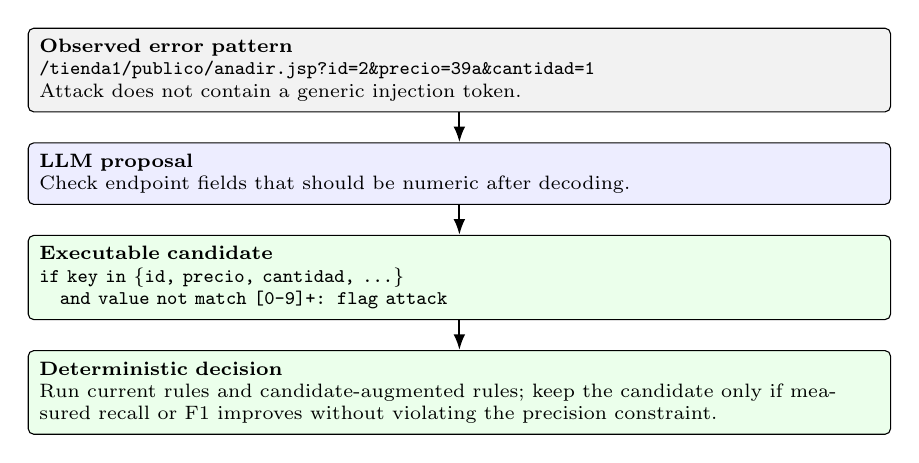
\begin{tikzpicture}[
    font=\scriptsize,
    node distance=0.38cm,
    box/.style={
        draw,
        rounded corners=2pt,
        align=left,
        text width=0.88\columnwidth,
        inner sep=4pt
    },
    data/.style={box, fill=gray!10},
    model/.style={box, fill=blue!7},
    eval/.style={box, fill=green!8},
    arrow/.style={-{Latex[length=2mm]}, thick}
]
\node[data] (error) {\textbf{Observed error pattern}\\
\texttt{/tienda1/publico/anadir.jsp?id=2\&precio=39a\&cantidad=1}\\
Attack does not contain a generic injection token.};
\node[model, below=of error] (proposal) {\textbf{LLM proposal}\\
Check endpoint fields that should be numeric after decoding.};
\node[eval, below=of proposal] (rule) {\textbf{Executable candidate}\\
\texttt{if key in \{id, precio, cantidad, ...\}}\\
\texttt{\quad and value not match [0-9]+: flag attack}};
\node[eval, below=of rule] (decision) {\textbf{Deterministic decision}\\
Run current rules and candidate-augmented rules; keep the candidate only if measured recall or F1 improves without violating the precision constraint.};

\draw[arrow] (error) -- (proposal);
\draw[arrow] (proposal) -- (rule);
\draw[arrow] (rule) -- (decision);
\end{tikzpicture}
\caption{Endpoint Invariants Catch Non-Obvious Attacks --- In this example, the LLM proposes a numeric-field invariant from sampled errors, but the harness decides whether the candidate becomes part of the detector by executing it and measuring its effect.}
\label{fig:method-example}
\end{figure}

Rule discovery is designed as an error-driven loop. The LLM inspects examples, summaries of retained rules, and sampled false positives and false negatives from the discovery side of the workflow. It then proposes a small batch of candidate rules, each with an intended field, pattern or heuristic, and expected failure mode. The process is iterative, but rule acceptance is based on measured behavior rather than on whether the rule sounds plausible. For the reported experiment, the resulting frozen rule set is evaluated on the held-out 20\% test split used by the machine-learning baseline.

Candidate rules are accepted only after execution. For each proposed batch, the harness evaluates the current rule set and the candidate-augmented rule set before deciding whether to retain it. A rule is kept only if it improves the chosen objective, such as F1 or recall, while satisfying an explicit precision constraint. Rules that merely duplicate existing detections, increase false positives beyond the threshold, or depend on brittle dataset artifacts are rejected. This makes acceptance empirical rather than conversational: a plausible explanation is not enough for a rule to enter the detector.

The final evaluation freezes the retained rules before measuring performance. Once the rule set is fixed, the harness evaluates the detector on the held-out test partition and reports accuracy, precision, recall, F1, and the confusion matrix. Runtime is measured separately from rule discovery because the discovery loop can involve LLM calls, human inspection, and repeated candidate evaluation. The deployment cost is only the cost of parsing each request and applying the compiled rules. This distinction is central to the method: the LLM may be expensive during discovery, but it is absent from inference.

The prototype is implemented as a lightweight Python harness. It uses standard CSV parsing to load CSIC 2010, \texttt{urllib.parse} to decode and parse request components, and Python's \texttt{re} engine to compile and apply regex rules. Each request is converted into a structured object before evaluation, and each retained rule records the field and pattern it inspects. We evaluate the frozen rule groups on the same stratified 80/20 split used by the machine-learning baseline. This keeps the reported comparison tied to held-out test requests rather than to aggregate full-dataset accuracy.

We also package the discovery process as an executable agent loop. The script presents the model with current metrics, sampled errors, and a catalog of candidate rule groups, then lets it choose the next group to evaluate. The model cannot write arbitrary detector code; it can only select from auditable candidate actions. The harness then executes the candidate and accepts it only if the measured objective improves while preserving the precision constraint. Algorithm~\ref{alg:agent-loop} shows the core control flow implemented by the reproducibility script.

\begin{algorithm}[t]
\caption{Candidate Rules Must Improve Metrics --- The agent loop accepts a planner-selected candidate only when deterministic evaluation shows that it preserves the precision constraint and improves the objective.}
\label{alg:agent-loop}
\begin{algorithmic}[1]
\State $S \gets$ empty rule state
\For{$i \gets 1$ to $R$}
    \State $m \gets \Call{Evaluate}{D_{\mathrm{dev}}, S}$
    \State $E \gets \Call{SampleErrors}{D_{\mathrm{dev}}, S}$
    \State $a \gets \textsc{PlannerChoose}(m, E, \mathcal{C} \setminus \textsc{Tried}(S))$
    \If{$a = \textsc{Stop}$}
        \State \textbf{break}
    \EndIf
    \State $S' \gets \Call{AddCandidate}{S, a}$
    \State $m' \gets \Call{Evaluate}{D_{\mathrm{dev}}, S'}$
    \If{$m'.\mathrm{precision} \ge p_{\min}$}
        \If{$m'.\mathrm{objective} > m.\mathrm{objective}$}
            \State $S \gets S'$
            \State \Call{Accept}{$a$}
        \Else
            \State \Call{Reject}{$a$}
        \EndIf
    \Else
        \State \Call{Reject}{$a$}
    \EndIf
\EndFor
\State \Return $S$
\end{algorithmic}
\end{algorithm}

\section{Dataset and Experimental Setup}

\subsection{Dataset}

We evaluate on the CSIC 2010 web-application attack dataset. The dataset contains HTTP requests for a synthetic online store, with each row labeled as either normal or anomalous. In the local CSV, the binary target appears both as a string label and as the numeric \texttt{classification} field, where 0 denotes normal traffic and 1 denotes anomalous traffic. Table~\ref{tab:dataset-summary} summarizes the local copy used in our experiments. The dataset is moderately imbalanced, but both classes are large enough to support the stratified 80/20 train/test split used in our comparison.

\begin{table}[t]
\centering
\begin{tabular}{lr}
\toprule
Property & Count \\
\midrule
Total requests & 61{,}065 \\
Normal requests & 36{,}000 \\
Anomalous requests & 25{,}065 \\
GET requests & 43{,}088 \\
POST requests & 17{,}580 \\
PUT requests & 397 \\
Rows with non-empty URL & 61{,}065 \\
Rows with non-empty body & 17{,}977 \\
\bottomrule
\end{tabular}
\caption{CSIC 2010 Provides a Balanced Web-Attack Benchmark --- The local CSV contains 61{,}065 labeled requests, including 36{,}000 normal requests and 25{,}065 anomalous requests from a synthetic online store.}
\label{tab:dataset-summary}
\end{table}

The CSV structure determines how requests are represented before rule evaluation. Each row contains HTTP headers, a \texttt{Method} field, a \texttt{URL} field, a request-body field named \texttt{content}, and a misspelled content-length field named \texttt{lenght}. GET requests store their payloads in the URL, while POST and PUT requests also carry non-empty bodies. We therefore treat URL and body as complementary evidence rather than assuming that all attack content appears in one place. Header fields are retained in the raw data, but the current detector focuses on method, URL, body, path, decoded text, and parsed parameters because those fields carry most of the request-specific variation.

\subsection{Baselines}

We compare the rule harness against a reproduced machine-learning baseline from a public Kaggle notebook for the same dataset. The baseline builds 18 numeric features from URL, body, method, and content-length properties, and it also constructs a character TF-IDF representation of the combined URL and body text. For the binary task, it trains a random forest on the numeric features plus 3{,}000 TF-IDF features. The notebook uses an 80/20 stratified train/test split with random seed 42, yielding 48{,}852 training requests and 12{,}213 test requests. We run this baseline locally with \texttt{uv} so that the comparison reflects the same dataset copy and machine environment.

The rule-based detector is evaluated separately from the machine-learning baseline. It parses each request into raw and decoded fields, compiles a fixed set of Python regexes, and applies both regex rules and deterministic endpoint heuristics. The final rule set contains 22 regex rules and 12 callback heuristics. We evaluate these frozen rules on the same stratified 80/20 split as the random-forest baseline, using random seed 42. The rule families were developed through iterative error analysis before this split-based reporting pass, so the result should be read as a held-out evaluation of a fixed detector rather than as a fully automated train-only discovery study.

\begin{table}[t]
\centering
\begin{tabular}{lp{1.95in}}
\toprule
Detector & Configuration \\
\midrule
Random forest & 18 numeric + char TF-IDF; 80/20 test \\
Regex harness & decoded fields + callbacks; 80/20 test \\
\bottomrule
\end{tabular}
\caption{Both Detectors Use the Same Held-Out Split --- The reproduced random forest and the frozen rule harness are evaluated on the same stratified 80/20 test split.}
\label{tab:experimental-configs}
\end{table}

\subsection{Evaluation Metrics}

We report standard binary-classification metrics. Accuracy measures the fraction of all requests classified correctly, while precision measures how often a request flagged as anomalous is actually anomalous. Recall measures how many anomalous requests are detected, and F1 summarizes the precision-recall tradeoff. We also report the confusion matrix because the operational meaning of a rule set depends on the balance between false positives and false negatives. This is especially important for deterministic rules, where a small number of broad patterns can improve recall while creating avoidable benign matches.

The split-based evaluation uses the same held-out test partition for both detector families. The random forest trains on 80\% of the data and reports binary performance on the remaining 20\%. The regex harness evaluates a frozen rule set on that same 20\% test split, which lets the comparison use the same test size and class balance. Candidate rule acceptance is still performed mechanically using precision and recall constraints, because regexes can overfit visible endpoint structure if tuned directly against final evaluation data.

\subsection{Runtime Measurement}

The rule harness is implemented as a small Python program. It loads the CSV with the standard \texttt{csv} module, decodes URL-encoded text with \texttt{urllib.parse}, parses query and body parameters with \texttt{parse\_qsl}, and applies compiled regular expressions with Python's \texttt{re} engine. Each request is converted into a structured object before evaluation, which avoids repeatedly reparsing the same fields while rules are applied. Runtime is measured in two parts: loading and request construction, and rule application over the constructed requests. This distinction lets us report both end-to-end runtime and the marginal cost of the detector once request objects exist.

The machine-learning baseline is implemented in the local notebook runner. It uses Pandas and scikit-learn to extract features, construct TF-IDF vectors, train the random forest, and save plots and model artifacts. We measure its script-level runtime from inside the runner and also record shell wall-clock time. These two runtimes answer different questions: the script timer captures the notebook pipeline after startup, while wall-clock time captures the cost of launching the full local run through \texttt{uv}. For the rule harness, the relevant deployment number is the time to parse requests and apply the frozen detector, since no LLM calls occur at inference time.

\section{Results}

\subsection{Rule-Set Performance}

The frozen rule set classifies nearly all held-out CSIC 2010 requests correctly. In its final round, the detector combines 22 regex rules with 12 deterministic endpoint heuristics. On the 20\% test split, it reaches 99.21\% accuracy, 99.92\% precision, 98.16\% recall, and 0.9903 F1. The confusion matrix in Table~\ref{tab:regex-confusion} shows that most remaining errors are false negatives rather than false positives. The close train/test match in Table~\ref{tab:regex-train-test} suggests that the retained rules capture repeated structure in the benchmark rather than only isolated examples.

\begin{table}[t]
\centering
\begin{tabular}{lrr}
\toprule
 & Predicted normal & Predicted attack \\
\midrule
Actual normal & 7{,}196 & 4 \\
Actual attack & 92 & 4{,}921 \\
\bottomrule
\end{tabular}
\caption{Most Remaining Errors Are False Negatives --- The final regex and heuristic rule set produces only four false positives on the held-out 20\% test split.}
\label{tab:regex-confusion}
\end{table}

\begin{table}[t]
\centering
\small
\begin{tabular}{lrrrrrr}
\toprule
Split & Acc. & Prec. & Rec. & F1 & FP & FN \\
\midrule
Train & 0.9920 & 0.9991 & 0.9815 & 0.9902 & 18 & 371 \\
Test & 0.9921 & 0.9992 & 0.9816 & 0.9903 & 4 & 92 \\
\bottomrule
\end{tabular}
\caption{Train and Test Performance Closely Match --- The frozen rule set reaches 99.21\% test accuracy and 0.9903 F1, with similar performance on the training partition.}
\label{tab:regex-train-test}
\end{table}

The rule iterations show that endpoint structure contributes more than obvious attack strings alone. Seed rules for script tags, SQL clusters, path traversal, and null bytes reached only 10.1\% held-out F1 because many anomalous requests do not contain a canonical injection token. Adding endpoint value checks and schema checks improved recall substantially by detecting malformed parameters, unexpected fields, and invalid endpoint-specific values. As shown in Figure~\ref{fig:accuracy-by-round}, test accuracy rises steadily as the loop adds endpoint-specific constraints after the initial generic signatures. This suggests that the LLM-guided loop is useful not merely for writing more signatures, but for identifying where endpoint-specific invariants make simple rules more precise.

\begin{figure}[t]
\centering
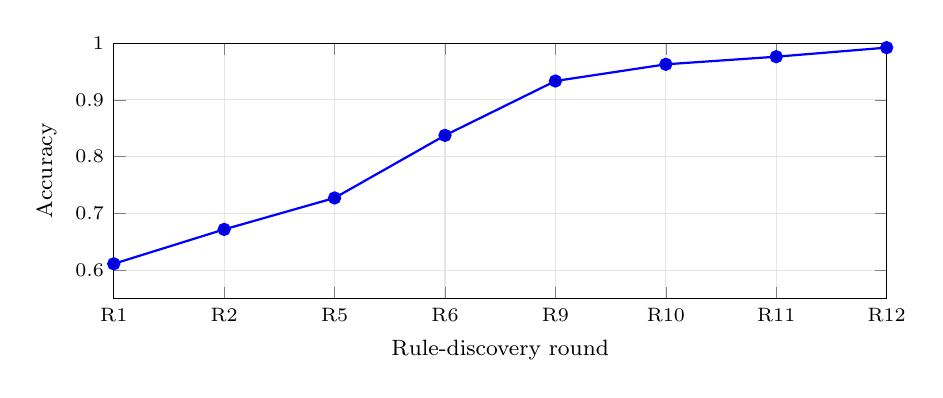
\begin{tikzpicture}
\begin{axis}[
    width=0.94\columnwidth,
    height=1.9in,
    ymin=0.55,
    ymax=1.0,
    xmin=1,
    xmax=8,
    ylabel={Accuracy},
    xlabel={Rule-discovery round},
    xtick={1,2,3,4,5,6,7,8},
    xticklabels={R1,R2,R5,R6,R9,R10,R11,R12},
    ytick={0.6,0.7,0.8,0.9,1.0},
    grid=both,
    grid style={gray!20},
    tick label style={font=\scriptsize},
    label style={font=\footnotesize},
    every axis plot/.append style={thick, mark=*}
]
\addplot coordinates {
    (1,0.6113)
    (2,0.6719)
    (3,0.7273)
    (4,0.8375)
    (5,0.9333)
    (6,0.9627)
    (7,0.9761)
    (8,0.9921)
};
\end{axis}
\end{tikzpicture}
\caption{Accuracy Improves as Rules Become More Structural --- Held-out test accuracy rises over successive LLM-guided rounds as the harness moves from obvious attack regexes to endpoint schemas, encoded payloads, static whitelisting, value constraints, identity-field checks, and contact/location heuristics.}
\label{fig:accuracy-by-round}
\end{figure}

\begin{table}[t]
\centering
\small
\begin{tabular}{lrrrr}
\toprule
Round & Acc. & Prec. & Rec. & F1 \\
\midrule
Seed rules & 0.6113 & 1.0000 & 0.0531 & 0.1008 \\
Schemas & 0.8375 & 0.9997 & 0.6042 & 0.7532 \\
Encoded & 0.9333 & 0.9998 & 0.8376 & 0.9115 \\
Values & 0.9627 & 0.9998 & 0.9092 & 0.9524 \\
Final rules & 0.9921 & 0.9992 & 0.9816 & 0.9903 \\
\bottomrule
\end{tabular}
\caption{Endpoint-Aware Rules Drive the Largest Gains --- Selected iterations show that schema, encoded-payload, value, and identity/contact heuristics substantially improve held-out F1 beyond seed attack signatures.}
\label{tab:rule-iterations}
\end{table}

\subsection{Comparison to Machine-Learning Baselines}

The reproduced machine-learning baseline confirms that CSIC 2010 is highly learnable from request text. The random forest baseline uses 18 numeric features together with character TF-IDF features over URL and body text. On its 20\% held-out split, it reaches 97.63\% accuracy, 0.9712 F1, and 0.9973 ROC-AUC on the binary task. These results provide a strong statistical baseline, but the detector is a trained model rather than a compact set of auditable request rules.

The regex rules are faster and more interpretable, and the split-based comparison puts both detectors on the same test size. Table~\ref{tab:model-comparison} reports the held-out binary results from the two local pipelines. The random forest reaches 97.63\% accuracy and 0.9712 F1, while the frozen regex harness reaches 99.21\% accuracy and 0.9903 F1. This comparison does not mean that regexes will dominate statistical models across settings. It shows that, on this structured benchmark, compact rules can match or exceed a strong text-based classifier while producing decisions that can be inspected rule by rule.

\begin{table}[t]
\centering
\begin{tabular}{lccc}
\toprule
Detector & Eval. & Acc. & F1 \\
\midrule
Random forest & 20\% test & 0.9763 & 0.9712 \\
Regex harness & 20\% test & 0.9921 & 0.9903 \\
\bottomrule
\end{tabular}
\caption{Rules Exceed the Reproduced ML Baseline on This Split --- The frozen rule harness reaches higher held-out accuracy and F1 than the reproduced random-forest pipeline on the same test partition.}
\label{tab:model-comparison}
\end{table}

The reproduced baseline also shows that feature choice matters. Numeric-only models perform substantially worse than the TF-IDF random forest, with the numeric-only random forest reaching 0.8931 accuracy and 0.8691 F1. Gradient boosting and logistic regression over the same numeric features perform lower still. This reinforces the same observation that motivates the rule harness: most of the useful evidence is in request text and request structure, not in coarse scalar summaries alone.

\subsection{Runtime}

The regex detector has a much smaller local pipeline cost than the reproduced machine-learning baseline. Applying the final rule set to all 61{,}065 requests took about 1.92 seconds after request construction, and the full load-parse-evaluate run took about 2.78 seconds. This corresponds to roughly 21{,}963 requests per second end to end on the local machine. The reproduced notebook reported 32.97 seconds of script runtime and 63.52 seconds of earlier shell wall-clock time for feature extraction, training, evaluation, and plot generation. These numbers are not identical deployment workloads, but they show the practical difference between a compiled rule set and a full model-training notebook pipeline.

\begin{table}[t]
\centering
\begin{tabular}{lr}
\toprule
Pipeline & Time \\
\midrule
Regex harness & 2.78 s \\
Reproduced ML baseline & 32.97 s \\
Reproduced ML baseline wall clock & 63.52 s \\
\bottomrule
\end{tabular}
\caption{Deterministic Rules Are Lightweight at Runtime --- The local rule harness processes the dataset much faster than the reproduced notebook pipeline, which includes feature extraction, training, evaluation, and plotting.}
\label{tab:runtime}
\end{table}

The runtime result is most relevant to the deployment setting. The LLM is not invoked when the final detector runs, and the regexes are compiled before evaluation. In contrast, the reproduced baseline includes training and artifact generation, so it is better understood as a baseline reproduction cost than as a pure inference benchmark. A follow-up measurement should separate trained-model inference from model training and plot generation. Even with that caveat, the current measurements show that the rule set can evaluate the entire dataset in seconds.

\subsection{Error Analysis}

The remaining regex errors mostly come from subtle endpoint-specific mutations. False negatives include anomalous requests where a parameter value is only slightly malformed, such as an identifier with an added slash or a password-like field containing unusual punctuation. These cases are difficult for broad injection signatures because they do not necessarily contain SQL, XSS, traversal, or shell tokens. They require knowledge of what values are valid for a particular endpoint and field. This is where the rule loop still has room to improve through split-aware endpoint invariants.

The false positives are few but informative. The final detector produces 4 false positives on the held-out test split, and earlier broad regexes show why precision can be fragile: benign address fields may contain apostrophes or punctuation that resembles injection syntax. This argues against accepting rules solely because they look plausible. It also motivates the metric-based acceptance discipline in the methodology, where a candidate rule must improve recall without introducing an unacceptable number of benign matches. In short, the error analysis supports the central design choice: rules should be proposed creatively, but accepted mechanically.

\section{Discussion}

The results suggest that simple rules can capture much of the structure in CSIC 2010. The strongest gains came from combining generic attack signatures with endpoint-specific expectations about paths, parameters, values, and field formats. This matters because many anomalous requests are not obviously malicious strings in isolation; they are malicious because they violate the local grammar of the application. A useful rule-discovery harness therefore needs to search for both attack syntax and application invariants.

The comparison to the machine-learning baseline is now made on the same 80/20 split. Both detectors report binary performance on the same held-out test size and class balance, which makes the accuracy and F1 comparison more direct than the earlier aggregate full-dataset run. The remaining caveat is about discovery, not evaluation: the rule families were developed through earlier error analysis before this split-based reporting pass. The regex result should therefore be interpreted as a held-out evaluation of a frozen detector, not as proof that a fully automated agent would rediscover the same rules from training data alone.

The main advantage of the rule set is that it is cheap and inspectable. The LLM is used to propose hypotheses, but every retained rule must survive deterministic evaluation and the final detector contains no model calls. When the detector makes a mistake, the triggering rule or missing invariant can be inspected directly. This makes the approach a plausible complement to heavier models in settings where models can help offline, but request-path detection should remain fast, stable, and auditable.

\section{Limitations}

The main limitation is about discovery provenance, not the reported test split. The final rule set is evaluated on the same held-out 20\% test split as the machine-learning baseline, so the reported accuracy and F1 respect the 80/20 evaluation protocol. However, the rule families were developed through earlier inspection of this dataset before the split-based reporting pass. A fully blinded agent study would freeze the split before any rule proposal begins and restrict all rule discovery to the training side.

The evaluation is also limited to one synthetic web application. CSIC 2010 is useful because it has stable endpoints, repeated parameter structure, and labeled attacks, but those same properties may make endpoint-specific rules easier to discover than they would be for a larger or more heterogeneous deployment. A rule set learned for this application should not be assumed to transfer directly to other applications, frameworks, or traffic distributions. Future work should evaluate whether the same harness can discover useful rules across multiple web-attack datasets and real application logs.

The method depends on careful rule-lifecycle management. Regexes and endpoint heuristics are interpretable, but they can still become brittle, redundant, or overly specific if accepted without constraints. Our harness reduces this risk by measuring candidate rules before retaining them, but it does not yet perform automated rule pruning, overlap detection, or long-term drift analysis. These mechanisms would be necessary before using the approach as a continuously updated operational rule set.

The runtime comparison is only a coarse comparison of local pipelines. The rule-harness runtime measures parsing and deterministic rule application, while the reproduced machine-learning baseline includes feature extraction, training, evaluation, and plot generation. This comparison is still useful for showing the cost difference between the current local workflows, but it is not a pure inference benchmark. A complete study should separately measure trained-model inference, feature extraction, rule matching, and LLM-assisted discovery time.

\section{Conclusion}

This paper studies whether an LLM can help discover web-attack detection rules without becoming the detector. We built a harness that uses the LLM only to propose regexes and endpoint heuristics, then relies on deterministic evaluation to decide which rules to retain. On the same stratified 80/20 split used by the reproduced random-forest baseline, the frozen rule set reached high held-out accuracy and ran over the full dataset in seconds. The result suggests that much of the benchmark's structure can be captured by auditable rules when generic attack signatures are combined with endpoint-specific invariants.

The broader takeaway is that LLMs may be useful in the rule-writing workflow even when they are unsuitable for the runtime detection path. A model can help search the space of candidate rules, but precision, recall, and rule acceptance should be enforced by a deterministic harness. This design preserves the benefits of simple rule engines: fast execution, stable behavior, and inspectable decisions. The next step is to run the discovery loop from scratch after freezing the split and to repeat the study across additional web-attack datasets.

\section*{Ethics}

This project uses a public benchmark dataset rather than live traffic or data collected from users. CSIC 2010 contains synthetic HTTP requests generated for a toy e-commerce application, so our experiments do not involve human subjects, private communications, or operational systems. The work is dual-use because attack-detection rules necessarily describe malicious request patterns. We limit that risk by studying benchmark classification and reproducibility rather than deployment against real services, and by reporting rules as defensive detection logic rather than attack instructions.

\section*{Author Contributions}

Rahul Tripathi and Armaan Oberai led the dataset inspection, rule-harness implementation, rule iteration, baseline reproduction, runtime measurement, and results analysis. Justine Ellery contributed to project framing, paper organization, writing review, and presentation preparation. All authors contributed to interpreting the results, refining the narrative, and preparing the final manuscript.

\section*{Reproducibility Artifacts}

The accompanying repository contains the CSIC 2010 CSV used in the experiments, the deterministic rule harness, the agent-loop harness, the split-based evaluation script, the reproduced Kaggle notebook runner, and a reproducibility README with exact commands. The main rule results can be regenerated with \texttt{uv run python} \path{project/regex_rules/evaluate_split.py}. The executable agent loop can be regenerated with \texttt{uv run python} \path{project/regex_rules/agent_rule_harness.py --planner replay}, or with an OpenAI API key using \path{--planner openai}. The reproduced machine-learning baseline can be regenerated with \texttt{uv run python} \path{project/kaggle_kernel/run_notebook25d16fa6ba_local.py}. These scripts use the local file \path{project/csic_database.csv} and the same stratified 80/20 split with random seed 42.

{\footnotesize

\bibliographystyle{acm}

\bibliography{sample}

}

\end{document}
